\documentclass[10pt]{beamer}

% ------------------------------------------------------------------------
% Carga del preámbulo personalizado
% (Recuerda colocar tu archivo preamble.tex en la misma carpeta,
%  con definiciones de temas, colores, macros, etc.)
% ------------------------------------------------------------------------
\usetheme[progressbar=frametitle]{metropolis}
\usepackage{appendixnumberbeamer}
\usepackage{fancyvrb}
\usepackage{booktabs}
\usepackage[scale=2]{ccicons}
\usepackage{pgfplots}
\usepgfplotslibrary{dateplot}
\usepackage{type1cm}
\usepackage{lettrine}
\usepackage{ragged2e}
\usepackage{xspace}
\newcommand{\themename}{\textbf{\textsc{metropolis}}\xspace}
\usepackage{graphicx} % Allows including images
\usepackage{booktabs} % Allows the use of \toprule, \midrule and \bottomrule in tables
\usepackage[utf8]{inputenc} %solucion del problema de los acentos.
\usepackage{xcolor}
\definecolor{LightGray}{gray}{0.9}

\usepackage{minted}
\usemintedstyle{tango}
\newcommand{\mypyfile}[1]{\inputminted[linenos=true, fontsize=\footnotesize, frame=lines, framesep=5\fboxrule,framerule=1pt]{python}{#1}}

\setminted[python]{breaklines,frame=lines,framesep=2mm,baselinestretch=1.2,bgcolor=LightGray,linenos, fontsize=\footnotesize} % obeytabs=true, tabsize=2, showtabs=true}

%%%%%%%%%%%%%%%%%%%%%%%%%%%%%%%%%%%%%%%%%%%%%%%%%%%%%%%%%%%%%%%%%%%%%%%%%%%%%%%%%%%%%%
\setbeamercolor{progress bar}{fg=blue!50!black,bg=white!50!black}
\setbeamercolor{title separator}{fg=red!50!black,bg=white!50!black}
\setbeamercolor{frametitle}{fg=white!80!black,bg=red!50!black}
\title[PCFI161]{Programaci\'on para F\'isica y Astronom\'ia}
\subtitle{Departamento de Física.}

\newcommand{\myfront}{
\author[PCFI161]{Corodinadora: C Loyola \\ Profesoras/es C Loyola / C Femenías / Y Navarrete / C Ruiz}
\institute[UNAB]{Universidad Andrés Bello}
\date{Primer Semestre 2025}
}

\titlegraphic{%
  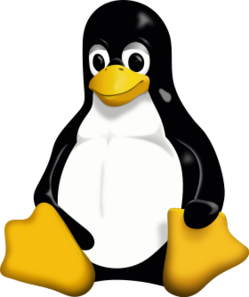
\includegraphics[width=.08\textwidth]{logo-tux.png}\hfill
  
\includegraphics[width=.3\textwidth]{logo-unab.png}\hfill
  
\includegraphics[width=.08\textwidth]{logo-python.png}
}

\makeatletter
\setbeamertemplate{title page}{
  \begin{minipage}[b][\paperheight]{\textwidth}
    \vfill%
    \ifx\inserttitle\@empty\else\usebeamertemplate*{title}\fi
    \ifx\insertsubtitle\@empty\else\usebeamertemplate*{subtitle}\fi
    \usebeamertemplate*{title separator}
    \ifx\beamer@shortauthor\@empty\else\usebeamertemplate*{author}\fi
    \ifx\insertdate\@empty\else\usebeamertemplate*{date}\fi
    \ifx\insertinstitute\@empty\else\usebeamertemplate*{institute}\fi
    \vfill
    \ifx\inserttitlegraphic\@empty\else\inserttitlegraphic\fi
    \vspace*{1cm}
  \end{minipage}
}
\makeatother


\makeatletter
\setlength{\metropolis@titleseparator@linewidth}{2pt}
\setlength{\metropolis@progressonsectionpage@linewidth}{2pt}
\setlength{\metropolis@progressinheadfoot@linewidth}{2pt}
\makeatother


\begin{document}

% ------------------------------------------------------------------------
% Portada personalizada (en tu preamble, podrías haber definido \myfront)
% ------------------------------------------------------------------------
\myfront{}

% ------------------------------------------------------------------------
% SLIDE 1: Título de la sesión (Semana 2, Sesión 1)
% Según el syllabus, esta vendría a ser la "Sesión 3"
% ------------------------------------------------------------------------
\begin{frame}[plain]
  \titlepage
  % Ajusta el título/subtítulo si quieres más detalle, por ejemplo:
  % \title{Semana 2 - Sesión 1 (Sesión 3): Sintaxis Básica de Python}
\end{frame}

% ------------------------------------------------------------------------
% SLIDE 2: Índice / Tabla de contenidos
% ------------------------------------------------------------------------
\begin{frame}
  \frametitle{Resumen - Semana 2, Sesión 1 (Sesión 3)}
  \tableofcontents
\end{frame}

% ------------------------------------------------------------------------
% Configuración de bloques (en caso de usar metrópolis, etc.)
% ------------------------------------------------------------------------
\metroset{block=fill}

% ----------------------------------------------------------------------------------------
% SECCIÓN 1: Contexto de la Sesión
% ----------------------------------------------------------------------------------------
\section{Introducción a la Sesión 3}

% ------------------------------------------------------------------------
% Slide 3: Objetivos de la Sesión
% ------------------------------------------------------------------------
\begin{frame}{Objetivos de la Sesión 3}
  \begin{itemize}
    \item \textbf{Introducir} las estructuras de control fundamentales en Python.
    \item \textbf{Dominar} el uso de condicionales (\texttt{if}, \texttt{elif}, \texttt{else}).
    \item \textbf{Comprender} bucles básicos (\texttt{for}, \texttt{while}) y su aplicación.
    \item \textbf{Aplicar} estas estructuras en problemas físicos y matemáticos.
    \item \textbf{Desarrollar} lógica de programación a través de ejercicios prácticos.
  \end{itemize}
\end{frame}

% ------------------------------------------------------------------------
% Slide 4: Conexión con la Sesión Anterior
% ------------------------------------------------------------------------
\begin{frame}{Conexión con Sesiones Previas}
  \begin{itemize}
    \item En la sesión anterior, exploramos la sintaxis básica de Python.
    \item Aprendimos sobre variables, tipos de datos y operaciones básicas.
    \item Ahora, construiremos sobre estos conceptos para manejar flujos de control.
  \end{itemize}
\end{frame}

% ----------------------------------------------------------------------------------------
% SECCIÓN 2: Estructuras de Control - Condicionales
% ----------------------------------------------------------------------------------------
\section{Estructuras de Control: Condicionales}

% ------------------------------------------------------------------------
% Slide 5: Introducción a las Estructuras Condicionales
% ------------------------------------------------------------------------
\begin{frame}{¿Qué son las Estructuras Condicionales?}
  \begin{itemize}
    \item Hasta ahora, nuestros programas ejecutan todas las líneas en \textbf{secuencia}.
    \item Las \textbf{estructuras condicionales} permiten que el programa tome \textbf{decisiones}.
    \item Ejecutan diferentes bloques de código según se cumplan ciertas \textbf{condiciones}.
  \end{itemize}
  
  \begin{block}{Analogía Física}
    Como un fotón que toma diferentes caminos según su energía: si \(E > E_{umbral}\) → efecto fotoeléctrico, sino → no hay emisión.
  \end{block}
\end{frame}

% ------------------------------------------------------------------------
% Slide 6: La Estructura IF Básica
% ------------------------------------------------------------------------
\begin{frame}[fragile]{La Estructura \texttt{if} Básica}
  \textbf{Sintaxis fundamental}:
  \begin{minted}{python}
if condición:
    # Código que se ejecuta SI la condición es True
    instrucción1
    instrucción2
  \end{minted}
  
  \textbf{Puntos clave}:
  \begin{itemize}
    \item La \texttt{condición} debe evaluarse como \texttt{True} o \texttt{False}.
    \item Los \textbf{dos puntos (:)} son obligatorios.
    \item La \textbf{indentación} (4 espacios) define qué código está dentro del \texttt{if}.
  \end{itemize}
\end{frame}

% ------------------------------------------------------------------------
% Slide 7: Ejemplo Práctico con IF
% ------------------------------------------------------------------------
\begin{frame}[fragile]{Ejemplo Práctico: Clasificación de Temperatura}
\begin{minted}{python}
temperatura = float(input("Temperatura del agua (°C): "))

if temperatura > 100:
    print("El agua está en estado gaseoso (vapor)")
    
if temperatura >= 0 and temperatura <= 100:
    print("El agua está en estado líquido")
    
if temperatura < 0:
    print("El agua está en estado sólido (hielo)")
\end{minted}

\textbf{Operadores de comparación}:
\begin{itemize}
  \item \texttt{>}, \texttt{<}, \texttt{>=}, \texttt{<=}, \texttt{==}, \texttt{!=}
  \item \texttt{and}, \texttt{or}, \texttt{not} para combinar condiciones
\end{itemize}
\end{frame}


% ------------------------------------------------------------------------
% Slide 8: La Estructura IF-ELIF-ELSE
% ------------------------------------------------------------------------
\begin{frame}[fragile]{La Estructura \texttt{if-elif-else} Completa}
  \textbf{Sintaxis mejorada para múltiples condiciones}:
  \begin{minted}{python}
if condición1:
    # Se ejecuta si condición1 es True
    código1
elif condición2:
    # Se ejecuta si condición1 es False y condición2 es True
    código2
elif condición3:
    # Se ejecuta si las anteriores son False y condición3 es True
    código3
else:
    # Se ejecuta si TODAS las condiciones anteriores son False
    código_por_defecto
  \end{minted}
  
  \textbf{Importante}: Solo se ejecuta \textbf{UNO} de los bloques (el primero que sea \texttt{True}).
\end{frame}


% ------------------------------------------------------------------------
% Slide 9: Ejemplo Mejorado con IF-ELIF-ELSE
% ------------------------------------------------------------------------
\begin{frame}[fragile]{Ejemplo Mejorado: Clasificación de Temperatura}
\begin{minted}{python}
temperatura = float(input("Temperatura del agua (°C): "))

if temperatura > 100:
    estado = "gaseoso (vapor)"
    energia = "alta"
elif temperatura >= 0:
    estado = "líquido"
    energia = "media"
else:  # temperatura < 0
    estado = "sólido (hielo)"
    energia = "baja"

print(f"A {temperatura}°C, el agua está en estado {estado}")
print(f"Nivel de energía cinética molecular: {energia}")
\end{minted}

\textbf{Ventaja}: Más eficiente y lógico que múltiples \texttt{if} independientes.
\end{frame}

% ----------------------------------------------------------------------------------------
% SECCIÓN 3: Estructuras de Control - Bucles
% ----------------------------------------------------------------------------------------
\section{Estructuras de Control: Bucles}

% ------------------------------------------------------------------------
% Slide 10: Introducción a los Bucles
% ------------------------------------------------------------------------
\begin{frame}{¿Qué son los Bucles?}
  \begin{itemize}
    \item Los \textbf{bucles} permiten repetir un bloque de código múltiples veces.
    \item Evitan la necesidad de escribir el mismo código una y otra vez.
    \item Python tiene dos tipos principales: \texttt{for} y \texttt{while}.
  \end{itemize}
  
  \begin{block}{Analogía Física}
    Como las órbitas planetarias: el planeta repite su trayectoria alrededor del sol hasta que alguna fuerza externa (condición) cambie el sistema.
  \end{block}
\end{frame}

% ------------------------------------------------------------------------
% Slide 11: El Bucle WHILE
% ------------------------------------------------------------------------
\begin{frame}[fragile]{El Bucle \texttt{while}}
  \textbf{Sintaxis}:
  \begin{minted}{python}
while condición:
    # Código que se repite MIENTRAS la condición sea True
    instrucción1
    instrucción2
    # IMPORTANTE: modificar algo para que eventualmente sea False
  \end{minted}
  
  \textbf{Características}:
  \begin{itemize}
    \item Se repite \textbf{mientras} la condición sea \texttt{True}.
    \item Si la condición nunca se vuelve \texttt{False} → \textbf{bucle infinito}.
    \item Útil cuando \textbf{no sabemos} cuántas repeticiones necesitamos.
  \end{itemize}
\end{frame}


% ------------------------------------------------------------------------
% Slide 12: Ejemplo Práctico con WHILE
% ------------------------------------------------------------------------

\begin{frame}{Ejemplo \\ Aproximación a la Raíz Cuadrada}
  \begin{block}{Enunciado}
    \begin{itemize}
      \item Calcular la raíz cuadrada de un número usando el método de Newton-Raphson.
      \item Usar la fórmula iterativa: $x_{n+1} = \frac{1}{2}(x_n + \frac{a}{x_n})$
      \item Usar un bucle \texttt{while} que continúe hasta que la precisión sea menor a 0.0001.
      \item Mostrar cada iteración y el resultado final.
      \item Verificar comparando con el valor real.
    \end{itemize}
  \end{block}
  
  \textbf{Conceptos:} Bucles \texttt{while}, precisión numérica, métodos iterativos.
  \\
  \textbf{Física relevante:} Métodos numéricos en simulaciones físicas.
\end{frame}

\begin{frame}[fragile]{Ejemplo: Aproximación a la Raíz Cuadrada (Método de Newton)}
\begin{minted}{python}
numero = float(input("Número para calcular raíz cuadrada: "))
aproximacion = numero / 2  # Estimación inicial
tolerancia = 0.0001

print(f"Calculando raíz cuadrada de {numero}...")

while abs(aproximacion**2 - numero) > tolerancia:
    aproximacion = (aproximacion + numero/aproximacion) / 2
    print(f"Aproximación actual: {aproximacion}")

print(f"Raíz cuadrada ≈ {aproximacion}")
print(f"Verificación: {aproximacion}² = {aproximacion**2}")
\end{minted}

\textbf{Física relevante}: Métodos iterativos son fundamentales en simulaciones físicas.
\end{frame}

% ------------------------------------------------------------------------
% Slide 13: El Bucle FOR con range()
% ------------------------------------------------------------------------
\begin{frame}[fragile]{El Bucle \texttt{for} con \texttt{range()}}
  \textbf{Sintaxis}:
  \begin{minted}{python}
for variable in range(inicio, fin, paso):
    # Código que se repite para cada valor de 'variable'
    instrucción1
    instrucción2
  \end{minted}
  
  \textbf{Ejemplos de range()}:
  \begin{itemize}
    \item \texttt{range(5)} → 0, 1, 2, 3, 4
    \item \texttt{range(1, 6)} → 1, 2, 3, 4, 5
    \item \texttt{range(0, 10, 2)} → 0, 2, 4, 6, 8
    \item \texttt{range(10, 0, -1)} → 10, 9, 8, 7, 6, 5, 4, 3, 2, 1
  \end{itemize}
  
  \textbf{Útil cuando}: Sabemos exactamente cuántas repeticiones necesitamos.
\end{frame}

% ------------------------------------------------------------------------
% Slide 14: Ejemplo Práctico con FOR
% ------------------------------------------------------------------------
\begin{frame}[fragile]{Ejemplo: Tabla de Conversión Celsius-Fahrenheit}
\begin{minted}{python}
print("Tabla de Conversión Celsius → Fahrenheit")
print("="*40)

for celsius in range(0, 101, 10):  # De 0°C a 100°C, cada 10°
    fahrenheit = (9/5) * celsius + 32
    print(f"{celsius:3d}°C = {fahrenheit:5.1f}°F")

print("="*40)
\end{minted}

\textbf{Salida esperada}:
\begin{verbatim}
  0°C =  32.0°F
 10°C =  50.0°F
 20°C =  68.0°F
 ...
100°C = 212.0°F
\end{verbatim}
\end{frame}


% ----------------------------------------------------------------------------------------
% SECCIÓN 4: Ejercicios Guiados
% ----------------------------------------------------------------------------------------
\section{Ejercicios Guiados}

% ------------------------------------------------------------------------
% Slide 15: Ejercicio 1 - Clasificador de Velocidades
% ------------------------------------------------------------------------
\begin{frame}{Ejercicio 1: \hfill \textcolor{red}{$\clubsuit$} \\ Clasificador de Velocidades}
  \begin{block}{Enunciado}
    Clasifique la velocidad de un objeto en función de su magnitud, considerando las siguientes categorías:
    \begin{itemize}
      \item \textbf{Movimiento lento}: Velocidad menor a 1 m/s.
      \item \textbf{Movimiento moderado}: Velocidad entre 1 y 10 m/s.
      \item \textbf{Movimiento rápido}: Velocidad entre 10 y 100 m/s.
      \item \textbf{Movimiento muy rápido}: Velocidad mayor a 100 m/s.
    \end{itemize}
    \textbf{Física relevante:} Escalas de velocidad en diferentes contextos físicos.
  \end{block}
\end{frame}



% ------------------------------------------------------------------------
% Slide 17: Ejercicio 2 - Suma de Números Pares
% ------------------------------------------------------------------------
\begin{frame}{Ejercicio 2: \hfill \textcolor{red}{$\clubsuit$} \\ Suma de Números Pares}
  \begin{block}{Enunciado}
    \begin{itemize}
      \item Calcular la suma de todos los números pares desde 2 hasta un número \(n\) dado por el usuario.
      \item Usar un bucle \texttt{for} con \texttt{range()}.
      \item Mostrar cada número par que se suma y el total final.
      \item Verificar el resultado usando la fórmula: $\sum_{k=1}^{n/2} 2k = n(n/2 + 1)$ para \(n\) par.
    \end{itemize}
  \end{block}
  
  \textbf{Conceptos:} Bucles \texttt{for}, acumuladores, validación matemática.
  \\
  \textbf{Física relevante:} Sumas de series son comunes en física estadística.
\end{frame}

% ------------------------------------------------------------------------
% Slide 19: Ejercicio 3 - Búsqueda de Número Secreto
% ------------------------------------------------------------------------
\begin{frame}{Ejercicio 3: \hfill \textcolor{red}{$\clubsuit$} \\ Juego de Adivinanza de Números}
  \begin{block}{Enunciado}
    \begin{itemize}
      \item El programa "piensa" en un número secreto entre 1 y 50.
      \item El usuario debe adivinar este número.
      \item Usar un bucle \texttt{while} que continúe hasta que el usuario acierte.
      \item Dar pistas: "muy cerca", "cerca", "alto", "bajo" según la proximidad.
      \item Contar el número de intentos y mostrar estadísticas al final.
    \end{itemize}
  \end{block}
  
  \textbf{Conceptos:} Bucles \texttt{while}, condicionales, contadores.
  \\
  \textbf{Física relevante:} Lógica de búsqueda y aproximación numérica.
\end{frame}

% ------------------------------------------------------------------------
% Slide 16: Solución 1 de Referencia - Clasificador de Velocidades
% ------------------------------------------------------------------------
\begin{frame}[fragile]{Solución 1 de Referencia: \hfill \textcolor{green}{$\checkmark$} \\ Clasificador de Velocidades}
\begin{minted}[fontsize=\tiny]{python}
# Entrada de datos
velocidad = float(input("Velocidad del objeto (m/s): "))
masa = float(input("Masa del objeto (kg, opcional, 0 si no aplica): "))

# Clasificación de velocidad
if velocidad < 1:
    categoria = "Movimiento lento"
elif velocidad < 10:
    categoria = "Movimiento moderado"
elif velocidad < 100:
    categoria = "Movimiento rápido"
else:
    categoria = "Movimiento muy rápido"

print(f"Velocidad: {velocidad} m/s → {categoria}")

# Cálculo de energía cinética si se proporciona masa
if masa > 0:
    energia_cinetica = 0.5 * masa * velocidad**2
    print(f"Energía cinética: {energia_cinetica} J")
\end{minted}
\textbf{Discusión:} Uso de condicionales anidadas y validación de entrada opcional.
\end{frame}

% ------------------------------------------------------------------------
% Slide 18: Solución 2 de Referencia - Suma de Números Pares
% ------------------------------------------------------------------------
\begin{frame}[fragile]{Solución 2 de Referencia: \hfill \textcolor{green}{$\checkmark$} \\ Suma de Números Pares}
\begin{minted}[fontsize=\tiny]{python}
# Entrada de datos
n = int(input("Ingrese el número límite: "))

# Inicializar acumulador
suma_pares = 0
print(f"Números pares desde 2 hasta {n}:")

# Bucle para sumar números pares
for numero in range(2, n + 1, 2):  # Desde 2, hasta n+1, de 2 en 2
    suma_pares += numero
    print(f"  + {numero}")

print(f"Suma total de números pares: {suma_pares}")

# Verificación con fórmula (solo si n es par)
if n % 2 == 0:
    formula_resultado = n * (n // 2 + 1)
    print(f"Verificación con fórmula: {formula_resultado}")
    print(f"¿Coinciden? {suma_pares == formula_resultado}")
\end{minted}
\textbf{Discusión:} Uso eficiente de range() con paso, acumuladores, y verificación matemática.
\end{frame}


% ------------------------------------------------------------------------
% Slide 20: Solución 3 de Referencia - Juego de Adivinanza
% ------------------------------------------------------------------------
\begin{frame}[fragile]{Solución 3 de Referencia: \hfill \textcolor{green}{$\checkmark$} \\ Juego de Adivinanza de Números}
\begin{minted}[fontsize=\tiny]{python}
# Número secreto: número entre 1 y 50
numero_secreto = 37
intentos = 0

print("¡Juego de adivinanza!")
print("He pensado en un número entre 1 y 50")
print("¿Puedes adivinarlo?")

while True:
    intento = int(input("Tu estimación: "))
    intentos += 1
    
    diferencia = abs(intento - numero_secreto)
    
    if intento == numero_secreto:
        print(f"¡Correcto! El número era {numero_secreto}")
        print(f"Lo lograste en {intentos} intentos")
        break
    elif diferencia <= 2:  # Muy cerca (diferencia de 1 o 2)
        print("¡Muy cerca!")
    elif diferencia <= 5:  # Cerca (diferencia de 3 a 5)
        print("Cerca...")
    elif intento < numero_secreto:
        print("Muy bajo")
    else:
        print("Muy alto")
\end{minted}
\textbf{Discusión:} Bucle infinito con \texttt{break}, rangos de proximidad progresivos, contadores de intentos.
\end{frame}


% ----------------------------------------------------------------------------------------
% SECCIÓN 5: Actividad Colaborativa
% ----------------------------------------------------------------------------------------
\section{Actividad Práctica}

% ------------------------------------------------------------------------
% Slide 21: Organización para Trabajo Grupal
% ------------------------------------------------------------------------
\begin{frame}{Organización para Trabajo en Equipos}
  \begin{block}{Formación de equipos}
    \begin{itemize}
      \item Grupos de 2-3 personas
      \item Cada persona crea su propio notebook
      \item Comparten pantalla y discuten soluciones
    \end{itemize}
  \end{block}
  
  \begin{block}{Metodología de trabajo}
    \begin{itemize}
      \item \textbf{10 min}: Lean y discutan los problemas
      \item \textbf{20 min}: Implementen las soluciones
      \item \textbf{5 min}: Prueben con diferentes valores
      \item \textbf{10 min}: Comparen resultados entre compañeros
    \end{itemize}
  \end{block}
\end{frame}

% ------------------------------------------------------------------------
% Slide 22: Actividad Extra 1 - Calculadora de Órbitas
% ------------------------------------------------------------------------
\begin{frame}{Actividad Extra 1: \hfill \textcolor{blue}{$\clubsuit$} \\ Calculadora de Período Orbital}
  \begin{block}{Enunciado}
    \begin{itemize}
      \item Calcular el período orbital de planetas usando la 3ª Ley de Kepler: $T^2 = \frac{4\pi^2}{GM}a^3$
      \item Pedir el semieje mayor \(a\) en metros.
      \item Usar \(G = 6.674 \times 10^{-11}\) m³/(kg·s²) y \(M_{sol} = 1.989 \times 10^{30}\) kg.
      \item Mostrar el período en segundos, días y años.
      \item Usar condicionales para clasificar el tipo de órbita.
    \end{itemize}
  \end{block}
  \textbf{Objetivo:} Integrar estructuras de control con cálculos astrofísicos.
\end{frame}

% ------------------------------------------------------------------------
% Slide 23: Actividad Extra 2 - Simulador de Decay Radioactivo
% ------------------------------------------------------------------------
\begin{frame}{Actividad Extra 2: \hfill \textcolor{blue}{$\clubsuit$} \\ Simulador de Decaimiento Radioactivo}
  \begin{block}{Enunciado}
    \begin{itemize}
      \item Simular el decaimiento radioactivo usando: $N(t) = N_0 e^{-\lambda t}$
      \item Pedir: número inicial de átomos $N_0$ y vida media $t_{1/2}$.
      \item Calcular $\lambda = \frac{\ln(2)}{t_{1/2}}$.
      \item Usar un bucle \texttt{for} para mostrar $N(t)$ cada 100 años hasta 1000 años.
      \item Agregar condicionales para alertar cuando quede menos del 10\% y 1\%.
    \end{itemize}
  \end{block}
  \textbf{Objetivo:} Bucles con aplicaciones en física nuclear.
\end{frame}

% ----------------------------------------------------------------------------------------
% SECCIÓN 6: Consolidación y Retroalimentación
% ----------------------------------------------------------------------------------------
\section{Consolidación y Retroalimentación}

% ------------------------------------------------------------------------
% Slide 24: Puesta en Común de Soluciones
% ------------------------------------------------------------------------
\begin{frame}{Puesta en Común - ¿Cómo les fue?}
  \textbf{Cada equipo comparta brevemente:}
  \begin{itemize}
    \item ¿Qué estructura de control les resultó más difícil de entender?
    \item ¿Encontraron errores comunes? ¿Cómo los solucionaron?
    \item ¿Algún truco o descubrimiento interesante con bucles o condicionales?
    \item ¿Cómo validaron que sus cálculos físicos fueran correctos?
  \end{itemize}
  
  \begin{alertblock}{Objetivo}
    Aprender de las experiencias de otros equipos y normalizar que los errores son parte del aprendizaje.
  \end{alertblock}
\end{frame}

% ------------------------------------------------------------------------
% Slide 25: Errores Comunes con Estructuras de Control
% ------------------------------------------------------------------------
\begin{frame}{Errores Comunes en Estructuras de Control}
  \begin{block}{Errores frecuentes con IF}
    \begin{itemize}
      \item Olvidar los dos puntos (:) después de la condición
      \item Problemas de indentación (usar tabs y espacios mezclados)
      \item Usar \texttt{=} (asignación) en lugar de \texttt{==} (comparación)
    \end{itemize}
  \end{block}
  
  \begin{block}{Errores frecuentes con bucles}
    \begin{itemize}
      \item \textbf{Bucle infinito}: No modificar la variable de control en \texttt{while}
      \item \textbf{Off-by-one}: Confusión con los límites de \texttt{range()}
      \item \textbf{Indentación}: No alinear correctamente el código dentro del bucle
    \end{itemize}
  \end{block}
  
  \begin{alertblock}{Consejo}
    Usar \texttt{print()} para debuggear: imprimir variables dentro de bucles para entender qué está pasando.
  \end{alertblock}
\end{frame}

% ----------------------------------------------------------------------------------------
% SECCIÓN 7: Conclusiones y Próximos Pasos
% ----------------------------------------------------------------------------------------
\section{Conclusiones}

% ------------------------------------------------------------------------
% Slide 26: Resumen de la Sesión
% ------------------------------------------------------------------------
\begin{frame}{Resumen de la Sesión}
  \begin{itemize}
    \item Dominamos las \textbf{estructuras condicionales} (\texttt{if}, \texttt{elif}, \texttt{else}).
    \item Aprendimos sobre \textbf{bucles} (\texttt{while}, \texttt{for}) y sus aplicaciones.
    \item Aplicamos estas estructuras a \textbf{problemas físicos reales}.
    \item Desarrollamos \textbf{lógica de programación} a través de ejercicios progresivos.
    \item Practicamos \textbf{debugging} y resolución colaborativa de problemas.
  \end{itemize}
  
  \begin{block}{Habilidad adquirida}
    Sus programas ahora pueden tomar decisiones inteligentes y automatizar tareas repetitivas.
  \end{block}
\end{frame}

% ------------------------------------------------------------------------
% Slide 27: Próximos Pasos
% ------------------------------------------------------------------------
\begin{frame}{Próximos Pasos}
  \begin{itemize}
    \item \textbf{Sesión 4 (Semana 2)}: Introducción a \textbf{funciones} en Python.
    \item \textbf{Temas futuros}:
      \begin{itemize}
        \item Definición de funciones y parámetros
        \item Reutilización de código y modularización
        \item Funciones en bibliotecas científicas
      \end{itemize}
    \item \textbf{Práctica recomendada}: Crear pequeños programas que combinen condicionales y bucles.
  \end{itemize}
  
  \begin{block}{Próxima sesión}
    Aprenderán a organizar su código en \textbf{funciones reutilizables} para resolver problemas más complejos.
  \end{block}
\end{frame}

% ------------------------------------------------------------------------
% Slide 28: Recursos Extra
% ------------------------------------------------------------------------
\begin{frame}{Recursos Extra}
  \begin{itemize}
    \item \href{https://docs.python.org/3/tutorial/controlflow.html}{\textbf{Python Docs - Control Flow}} (documentación oficial).
    \item \href{https://realpython.com/python-conditional-statements/}{\textbf{Real Python - Conditionals}} (tutoriales avanzados).
    \item \href{https://realpython.com/python-for-loop/}{\textbf{Real Python - For Loops}} (ejemplos prácticos).
    \item \href{https://www.learnpython.org/en/Loops}{\textbf{LearnPython.org - Loops}} (ejercicios interactivos).
  \end{itemize}
  
  \begin{block}{Práctica adicional}
    Prueben modificar los ejercicios de hoy agregando más condicionales o cambiando los rangos de los bucles.
  \end{block}
\end{frame}

% ------------------------------------------------------------------------
% Slide 29: Entrega y Recursos
% ------------------------------------------------------------------------
\begin{frame}{Entrega de Trabajo y Recursos}
  \begin{block}{Entrega (Canvas)}
    \begin{itemize}
      \item Sube tu notebook con los 3 ejercicios principales resueltos
      \item Incluye comentarios explicando tu razonamiento
      \item Al menos una de las actividades extra completada
      \item Fecha límite: antes de la próxima clase
    \end{itemize}
  \end{block}
  
  \begin{block}{Autoevaluación}
    \begin{itemize}
      \item ¿Entiendo cuándo usar \texttt{if-elif-else} vs múltiples \texttt{if}?
      \item ¿Sé cuándo elegir \texttt{for} vs \texttt{while}?
      \item ¿Puedo debuggear bucles infinitos?
    \end{itemize}
  \end{block}
\end{frame}

% ------------------------------------------------------------------------
% Slide 30: Cierre Motivacional
% ------------------------------------------------------------------------
\begin{frame}
  \huge{\centerline{¡Excelente progreso!}}
  \vspace{0.5cm}
  \normalsize
  \begin{itemize}
    \item Ahora dominan las \textbf{estructuras de control fundamentales}
    \item Sus programas pueden \textbf{tomar decisiones} y \textbf{automatizar tareas}
    \item Están listos para \textbf{funciones} y \textbf{modularización}
    \item Recuerden: \textbf{la práctica constante} es clave
  \end{itemize}
  
  \begin{center}
    \textbf{¡Nos vemos en la Sesión 4!}
  \end{center}
\end{frame}

\end{document}
